\documentclass[portrait,a4paper]{article}


\usepackage[utf8x]{inputenc}
\usepackage[T1]{fontenc}


\usepackage{mathtools}
\usepackage{amssymb,amsfonts,amsmath}
\usepackage[e]{esvect}

\usepackage{algorithmic}
\usepackage{algorithm}
\newcommand{\algorithmlabel}[2]{{
    \renewcommand{\algorithmicensure}{\textbf{#1}:}
    \ENSURE{#2~}
}}

\usepackage{graphicx}
\usepackage[svgnames]{xcolor}

\usepackage{geometry}
\geometry{a4paper}

% multirow and multicol
\usepackage{multirow}
\usepackage{multicol}
\columnsep24pt
\columnseprule0.1pt

% enumerate
\renewcommand\theenumi{\arabic{enumi}}
\renewcommand\labelenumi{\theenumi.}
\renewcommand\theenumii{\roman{enumii}}
\renewcommand\labelenumii{\theenumii)}

\usepackage{listings}
\lstset{
    floatplacement={tbp},
    basicstyle=\ttfamily\mdseries,
    identifierstyle=,
    stringstyle=\color{gray},
    numbers=left,
    numbersep=5pt,
    inputencoding=utf8x,
    xleftmargin=8pt,
    xrightmargin=8pt,
    keywordstyle=[1]\bfseries,
    keywordstyle=[2]\bfseries,
    keywordstyle=[3]\bfseries,
    keywordstyle=[4]\bfseries,
    numberstyle=\tiny,
    stepnumber=1,
    breaklines=true,
    frame=lines,
    showstringspaces=false,
    tabsize=2,
    commentstyle=\color{gray},
    captionpos=b,
    float=float,
    language={Java}
}
\newcommand{\code}[1]{\lstinline{#1}}

% hyperref
\usepackage[colorlinks=true,pdfborder={0 0 0},citecolor=DarkGreen,linkcolor=DarkBlue,urlcolor=DarkBlue]{hyperref}

% depth of section numbering
\setcounter{secnumdepth}{4}

% redefine the \paragraph command:
\makeatletter
\renewcommand\paragraph{\@startsection{paragraph}{4}{0mm}%
    {-\baselineskip}%
    {0.5\baselineskip}%
    {\normalfont\bfseries}%
}%
\makeatother

% new chapter command
\newcommand{\newchapter}{\clearpage\pagebreak}

% theorems
\usepackage{amsthm}
\newtheorem{lemma}{Lemma}[section]
\newtheorem{theorem}{Theorem}[section]
\newtheorem{corollary}{Corollary}[section]
\newtheorem{definition}{Definition}[section]
\newtheorem{remark}{Remark}[section]
\newtheorem{observation}{Observation}[section]
\newtheorem{assumption}{Assumption}[section]
\newtheorem{proposition}{Proposition}[section]

% autoref names
\newcommand{\specialref}[2]{\hyperref[#1]{#2~\ref*{#1}}}
\def\lstlistingautorefname{Listing}
\def\subsubsectionautorefname{Section}
\def\subsectionautorefname{Section}
\def\figureautorefname{Figure}

% parindent
\parindent0px
\parskip3pt

% redefine greek letters
\renewcommand{\phi}{\varphi}
\renewcommand{\epsilon}{\varepsilon}

% shortcuts in math mode
% \newcommand{\bs}{\boldsymbol}
\newcommand{\mc}{\mathcal}
\newcommand{\ds}{\displaystyle}
\DeclarePairedDelimiter\absimpl{\lvert}{\rvert}
\DeclarePairedDelimiter\normimpl{\lVert}{\rVert}
\newcommand{\abs}[1]{\absimpl*{#1}}
\newcommand{\norm}[1]{\normimpl*{#1}}
\newcommand{\argmax}{\operatorname*{arg\,max}}
\newcommand{\argmin}{\operatorname*{arg\,min}}

% number sets
\newcommand{\R}{\mathbb{R}}
\newcommand{\Z}{\mathbb{Z}}
\newcommand{\N}{\mathbb{N}}
\newcommand{\Q}{\mathbb{Q}}
\newcommand{\C}{\mathbb{C}}
\newcommand{\F}{\mathbb{F}}
\newcommand{\LL}{\mathcal{L}}
\newcommand{\powerset}{\mathcal P}

% probabilities
\newcommand{\Prob}[1]{\operatorname{Pr}\left[#1\right]}
\newcommand{\Ex}[1]{\mathbb{E}\left[#1\right]}

% misc
\newcommand{\bigO}[1]{\mc O\left(#1\right)} % big-o notation

\newcommand{\nop}[1]{} % temporarily remove from output




% todo
\usepackage{framed}
\newenvironment{todo}
{\color{DarkRed} \begin{leftbar}}
{\end{leftbar}}
\newcommand{\inlinetodo}[1]{{\textcolor{DarkRed}{ [\textbf{TODO}: #1]}}}
\newcommand{\mat}[1]{\bs{#1}}
\newcommand{\ma}{\mat{A}}
\newcommand{\mb}{\mat{B}}
\newcommand{\mx}{\mat{X}}
\newcommand{\mv}{\mat{V}}
\newcommand{\muu}{\mat{U}}
\newcommand{\md}{\mat{D}}
\newcommand{\ms}{\mat{S}}
\newcommand{\mz}{\mat{Z}}

\newcommand{\vx}{\mat{x}}
\newcommand{\va}{\mat{a}}
\newcommand{\vb}{\mat{b}}
\newcommand{\vu}{\mat{u}}
\newcommand{\vz}{\mat{z}}

\newcommand{\rd}{\R^D}
\newcommand{\rr}[2]{\R^{#1 \times #2}}

\usepackage{placeins}

\newcommand*{\titleSW}[3]{\begingroup% Story of Writing
\raggedleft
\vspace*{\baselineskip}
{\Huge\textbf{#1}}\\[0.7\baselineskip]
{\large\textbf{#2}}\\[0.5\baselineskip]
{\small #3}\par
\endgroup}

\begin{document}

 \author{Pascal Spörri\\pascal@spoerri.io}
 \title{HOWTO WRITE FAST NUMERICAL CODE\\ EXERCISE 6}
 \date{\today}
\maketitle

\section{Warmup}
The code of this exercise has been run on an Intel Core i5-3570K CPU and Ubuntu 12.04 with gcc 4.6.3.
\lstinputlisting[caption=Code of \lstinline{base.c}]{warmup/base.c}

\subsection{Baseline}
The code of \lstinline{base.c} has been compiled with the compiler flags: \lstinline{-m64 -march=corei7-avx -fno-tree-vectorize -O3 -S}.
\paragraph{Assembly code:} 
%\lstset{language=asm}

\lstinputlisting[caption=Compiler output of \lstinline{base.c} using the flags \lstinline{-m64 -march=corei7-avx -fno-tree-vectorize -O3 -S}]{warmup/base.asm}

We observe that no vector instructions have been used.

\subsection{Autovectorization}
The code of \lstinline{auto.c} has been compiled with the compiler flags: \lstinline{-m64 -march=corei7-avx -O3 -S}.

\lstinputlisting[caption=Compiler output of \lstinline{auto.c} using the flags \lstinline{-m64 -march=corei7-avx -O3 -S}]{warmup/auto.asm}
We observe that the code contains multiple versions of the basecode. One vectorised version that uses SSE and one non vectorised version that uses non-SSE code. The code tries to select the optimal variant.

\subsection{Manual Vectorization}
We decided to implement the manual step using AVX registers:
\lstinputlisting{warmup/manual.c}
%manual.c
%{'num_runs': 262144, 'total_sum': 1.369678, 'cycles': 754.563652, 'flops_cycle': 3.180646, 'size': 800}
%base.c
%{'num_runs': 32768, 'total_sum': 1.369678, 'cycles': 5115.335144, 'flops_cycle': 0.469177, 'size': 800}
%auto.c
%{'num_runs': 131072, 'total_sum': 1.369678, 'cycles': 1256.937363, 'flops_cycle': 1.909403, 'size': 800}

\subsection{Performance}
\begin{figure}[H]
\centering
\begin{tabular}{rlll}
    \textbf{Code} & \textbf{Flops/Cycle} & \textbf{Speedup} & \textbf{Compiler Flags}\\ 
        \texttt{base.c} & $0.469$ & Baseline & \texttt{-m64 -march=corei7-avx -fno-tree-vectorize -O3}\\
    \texttt{auto.c} & $1.909$ & $4.07x$ & \texttt{-m64 -march=corei7-avx -O3}\\
    \texttt{manual.c}& $3.18$ & $6.78x$ & \texttt{-m64 -march=corei7-avx -O3}
\end{tabular}
    \caption{Baseline comparison on an Intel Core i5-3570K CPU, Ubuntu 12.04 with gcc 4.6.3. Inputsize: 800}\label{warmup_performance}
\end{figure}

We observe a $6.78x$ speedup with respect to our the non-vectorized implementation and a $1.67x$ speedup with repsect to our auto vectorized implementation. 

\begin{figure}[H]
    \centering
    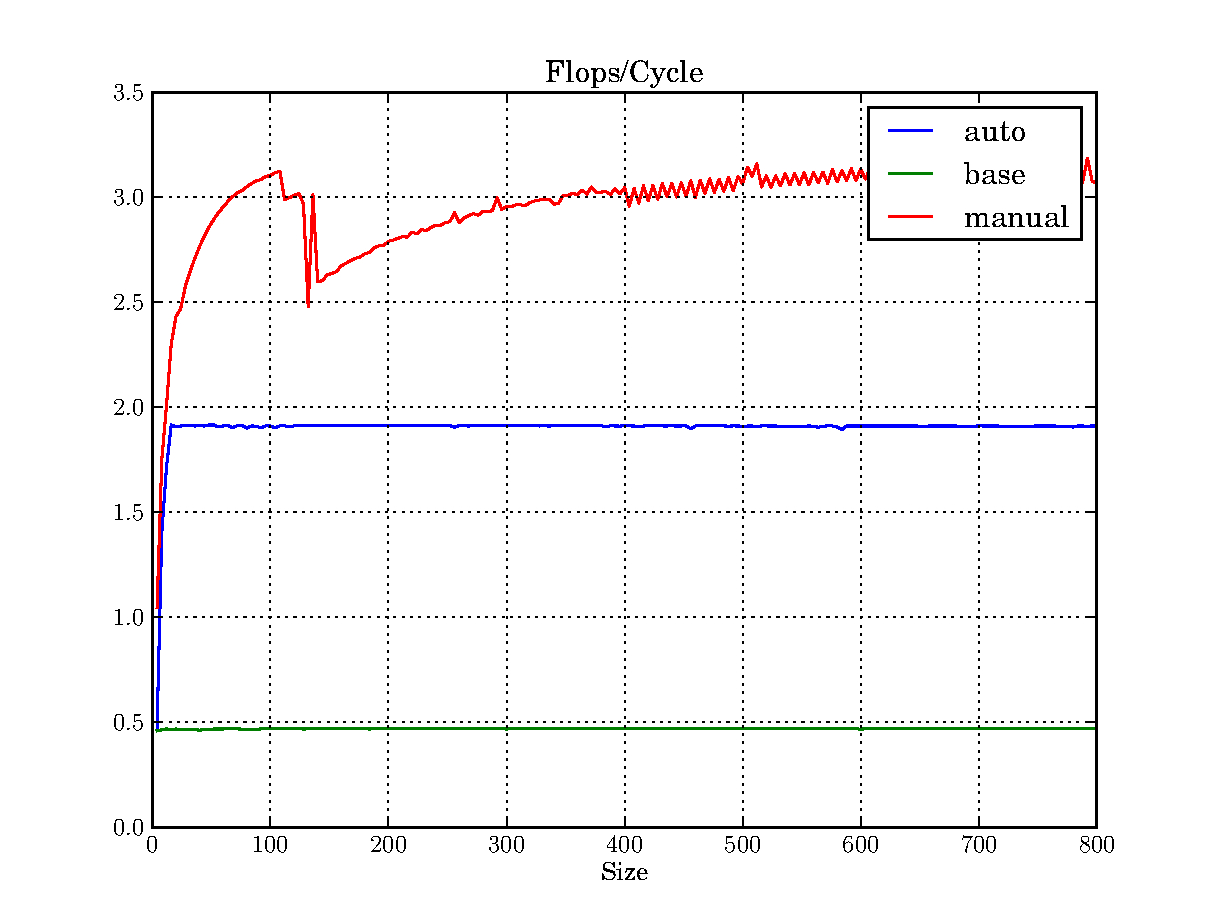
\includegraphics[width=0.75\textwidth]{warmup/plot.pdf}
    \caption{Comparsion plot of \lstinline{base.c}, \lstinline{auto.c} and \lstinline{manual.c} using the compiler options described in figure \ref{warmup_performance} on an Intel Core i5-3570K CPU and Ubuntu 12.04 with gcc 4.6.3.}
\end{figure}

%%%%%%%%%%%%%%%%

\section{Vectorization}
The code of this exercise has been run on an Intel Core i5-3570K CPU and Ubuntu 12.04 with gcc 4.6.3.
\lstinputlisting[caption=Code of \lstinline{base.c}]{vectorization/base.c}

\subsection{Baseline}
The code of \lstinline{base.c} has been compiled with the compiler flags: \lstinline{-m64 -march=corei7-avx -fno-tree-vectorize -O3 -S}.
\paragraph{Assembly code:} 
\lstinputlisting[caption=Compiler output of \lstinline{base.c} using the flags \lstinline{-m64 -march=corei7-avx -fno-tree-vectorize -O3 -S}]{vectorization/base.asm}

We observe that no vector instructions have been used.
%%%

\subsection{Autovectorization}
The code of \lstinline{auto.c} has been compiled with the compiler flags: \lstinline{-m64 -march=corei7-avx -O3 -S}.

\lstinputlisting[caption=Compiler output of \lstinline{auto.c} using the flags \lstinline{-m64 -march=corei7-avx -O3 -S}]{vectorization/auto.asm}
We note that the compiler made heavy use of AVX instructions. The code also contains a loop version that works with arbitrary input sizes. 

\subsection{Manual Vectorization}
Based on the output of the automatic vectorization we decided to implement a first version using AVX registers:
\lstinputlisting[caption=First version of the manual vectorization (\lstinline{manual.c}).]{vectorization/manual.c}
Since this version of code didn't provide any speedup compared to our non vectorized implementation (see figure \ref{vectorization_performance}) we decided to implement a version using SSE instructions:
\lstinputlisting[caption=Version of the manual vectorization using SSE instructions (\lstinline{manual3.c}).]{vectorization/manual3.c}
Using this version we were better than our baseline but still slower than the automatically generated vectorization (see figure \ref{vectorization_performance}).

For our final version we decided to replace the \lstinline{_mm_alignr_epi8} expressions with \lstinline{_mm_loadu_ps} expressions:
\lstinputlisting[caption=Improved code based on \lstinline{manual3.c} (\lstinline{manual4.c}).]{vectorization/manual4.c}
Using this code we were able to improve the our manually tuned code. We were able to achieve a $3.36x$ speedup compared to our baseline (see figure  \ref{vectorization_performance}).

\subsection{Performance}
%manual3.c
%main.c: In function 'malloc_aligned':
%main.c:55:13: warning: cast to pointer from integer of different size [-Wint-to-pointer-cast]
%{'num_runs': 131072, 'total_sum': 10.0, 'cycles': 929.474274, 'flops_cycle': 6.024911, 'size': 800}
%manual4.c
%main.c: In function 'malloc_aligned':
%main.c:55:13: warning: cast to pointer from integer of different size [-Wint-to-pointer-cast]
%{'num_runs': 131072, 'total_sum': 10.0, 'cycles': 867.609406, 'flops_cycle': 6.454517, 'size': 800}
%manual.c
%main.c: In function 'malloc_aligned':
%main.c:55:13: warning: cast to pointer from integer of different size [-Wint-to-pointer-cast]
%{'num_runs': 65536, 'total_sum': 10.0, 'cycles': 2922.041077, 'flops_cycle': 1.916469, 'size': 800}
%base.c
%main.c: In function 'malloc_aligned':
%main.c:55:13: warning: cast to pointer from integer of different size [-Wint-to-pointer-cast]
%{'num_runs': 65536, 'total_sum': 10.0, 'cycles': 2912.57077, 'flops_cycle': 1.9227, 'size': 800}
%auto.c
%main.c: In function 'malloc_aligned':
%main.c:55:13: warning: cast to pointer from integer of different size [-Wint-to-pointer-cast]
%{'num_runs': 131072, 'total_sum': 10.0, 'cycles': 842.677155, 'flops_cycle': 6.645487, 'size': 800}

\begin{figure}[H]
\centering
\begin{tabular}{rlll}
    \textbf{Code} & \textbf{Flops/Cycle} & \textbf{Speedup} & \textbf{Compiler Flags}\\ 
        \texttt{base.c} & $1.92$ & Baseline & \texttt{-m64 -march=corei7-avx -fno-tree-vectorize -O3}\\
    \texttt{auto.c} & $6.65$ & $3.45x$ & \texttt{-m64 -march=corei7-avx -O3}\\
    \texttt{manual.c}& $1.92$ & $1.00x$ & \texttt{-m64 -march=corei7-avx -O3}\\
    \texttt{manual3.c}& $6.02$ & $3.13x$ & \texttt{-m64 -march=corei7-avx -O3}\\
    \texttt{manual4.c}& $6.45$ & $3.36x$ & \texttt{-m64 -march=corei7-avx -O3}
\end{tabular}
    \caption{Baseline comparison on an Intel Core i5-3570K CPU, Ubuntu 12.04 with gcc 4.6.3.}\label{vectorization_performance}
\end{figure}

We observe a $3.36x$ speedup with our \lstinline{manual4.c} code (compiled with \texttt{-m64 -march=corei7-avx -O3} using GCC 4.6.3) compared to the non-vectorized baseline \lstinline{base.c} (compiled with \texttt{-m64 -march=corei7-avx -fno-tree-vectorize -O3} using GCC 4.6.3). A performance plot has been provided here: 
\begin{figure}[H]
    \centering
    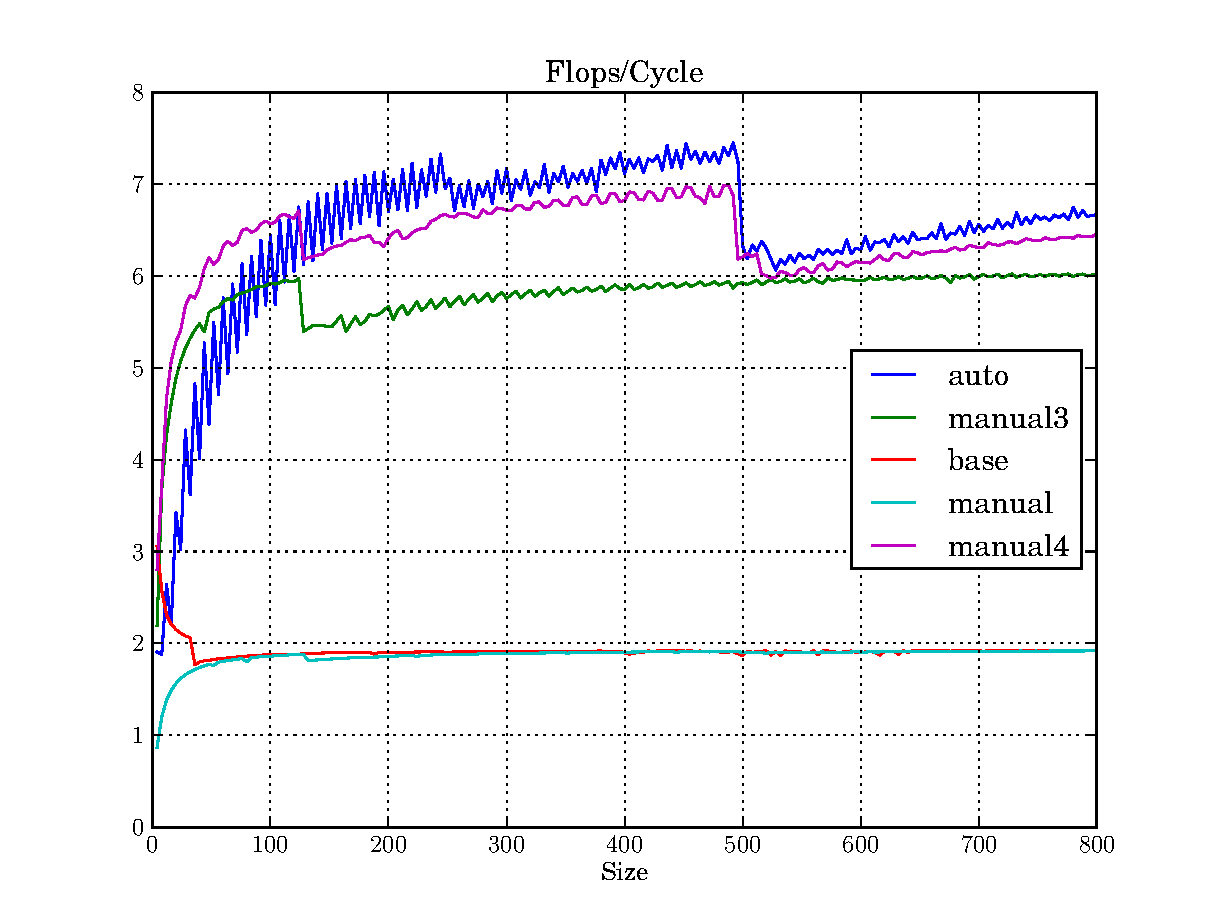
\includegraphics[width=0.75\textwidth]{vectorization/plot.pdf}
    \caption{Comparsion plot of \lstinline{base.c}, \lstinline{auto.c} and \lstinline{manual.c} using the compiler options described in figure \ref{vectorization_performance} on an Intel Core i5-3570K CPU and Ubuntu 12.04 with gcc 4.6.3.}
\end{figure}
\end{document}